\begin{singlespacing}
\begin{figure}[H]
\centering
  \captionsetup{justification=left}
    {\captionsetup{justification=centering,singlelinecheck=off}
\caption{\bfseries Time series plots of the posterior means of the time-varying relation between six-factor alphas and characteristics $\delta_t$} \label{figure1} } 
\caption*{The figure presents estimation results of the model in Eqs.(\ref{asset}), (\ref{cross}) and (\ref{delta_t}) examining the cross-sectional relation between six-factor alphas and all characteristics simultaneously. In each plot we report posterior results for a given characteristic across our sample period February 2001 to December 2016. The solid line is the posterior mean of $\delta_t$ and the dashed lines represent the 95\% credible interval.}
  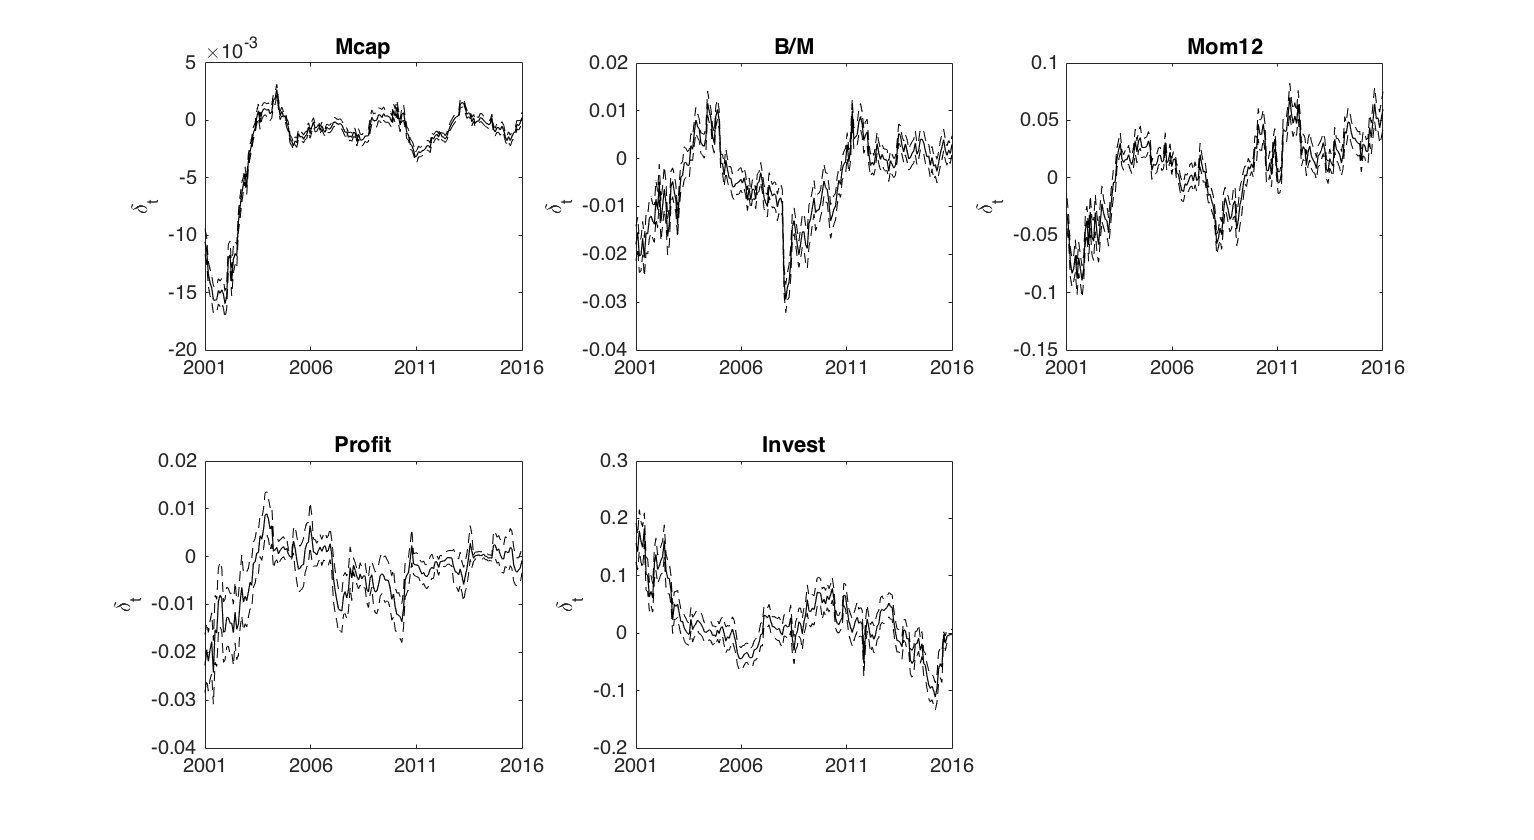
\includegraphics[width=18cm,height=10cm,\textwidth]{pictures/posterior_plots.png}

\end{figure}
\end{singlespacing}

\begin{singlespacing}
\begin{figure}[H]
\centering
  \captionsetup{justification=left}
  {\captionsetup{justification=centering,singlelinecheck=off}
  \caption{\bfseries Cumulative alphas for top-minus-bottom portfolios }\label{figure2} } 
\caption*{This figure presents the cumulative post-ranking Fama-French six-factor alpha for top-minus-bottom portfolios sorted on one of the following performance measures: six-factor alpha ($\alpha$), double-adjusted six-factor alpha ($\alpha^*$), or characteristic-driven performance ($\alpha^{char}$). These performance measures are calculated using rolling windows with a window size of 24 months. Portfolios are rebalanced every quarter-end and held up to 40 quarters. The horizontal axis shows the post-ranking holding period in quarters.}
  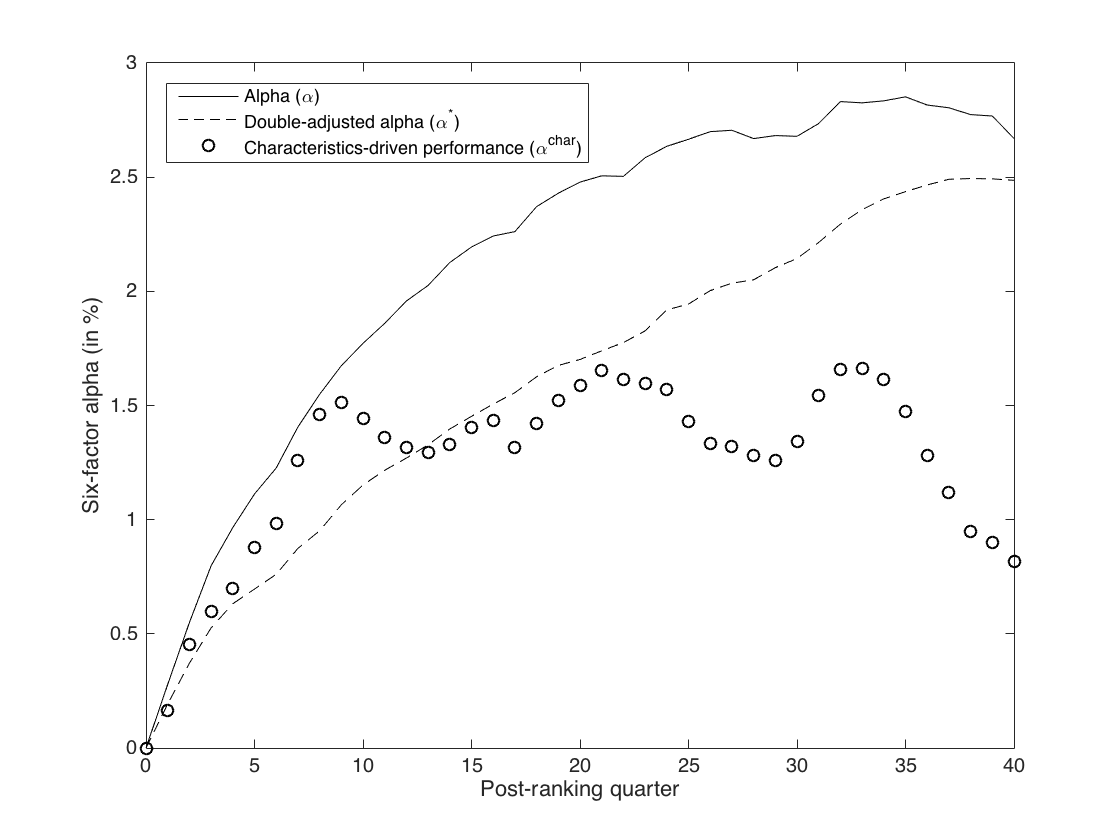
\includegraphics[width=14cm,height=7cm,\textwidth]{pictures/persistence.png}

\end{figure}
\end{singlespacing}
